The results from these simulations unequivocally demonstrated that without the ``Sequential Saturation'' logic discovered by the artificial intelligence, no amount of static rebalancing between Education, Enforcement, or Incentives was sufficient to resolve the municipality-wide non-compliance problem \citep{Jimenez2025, ZhengAI2022}.

\subsection{Baseline: The Status Quo}

To establish a comparative baseline, the simulation first evaluated the current administrative strategy employed by the Local Government Unit (LGU). Under this ``Status Quo'' regime, the Mayor Agent acts purely as a passive distributor, dividing the \textpeso 375,000 quarterly municipal budget equally among all seven barangays. As verified by the telemetry logs, this resulted in a fixed augmentation of exactly \textpeso 53,571.43 per node (14.3\% of the budget), with 100\% of these municipal funds allocated strictly to Information, Education, and Communication (IEC) campaigns under the assumption that passive awareness drives compliance.

The simulation results over the 12-quarter (3-year) horizon revealed a profound structural failure in this equal-distribution strategy. As illustrated in Figure \ref{fig:baseline_graph}, the Global Compliance Rate (the black trajectory) suffered from severe stagnation, artificially ceiling at approximately 30.18\% by Quarter 12. 

\begin{figure}[htbp]
\centering
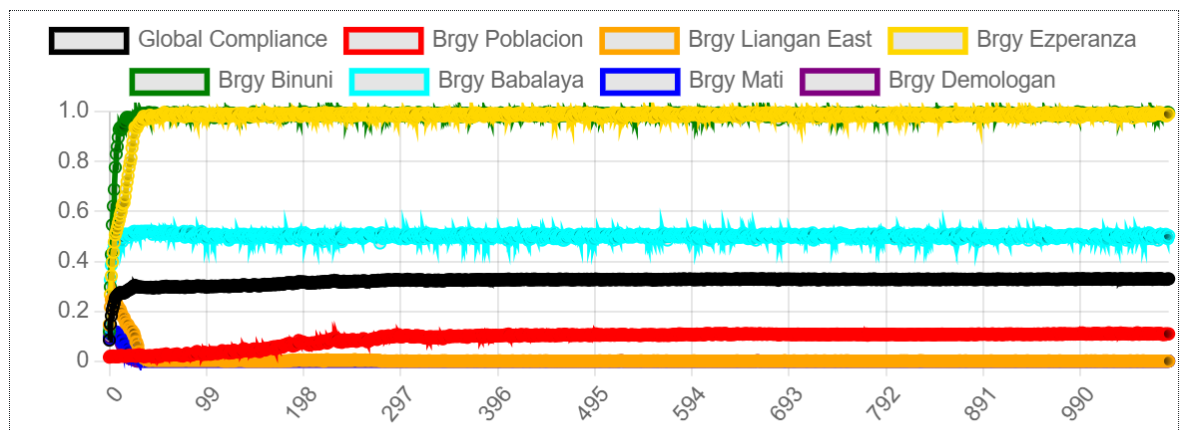
\includegraphics[width=\textwidth]{images/Baseline.png}
\caption{Comparative compliance trajectories under the Status Quo strategy, illustrating the severe bifurcation between low-density and high-density barangays.}
\label{fig:baseline_graph}
\end{figure}

However, analyzing the localized data reveals that this 30\% global stagnation is not the result of uniform municipal failure, but rather a violent computational bifurcation driven by Population Density Bias:

\begin{itemize}
    \item \textbf{The Success of the Small (Over-funding):} The equal injection of \textpeso 53,571.43 proved highly effective for the municipality's least populated sectors. Barangays Mati ($N=165$), Babalaya ($N=171$), Demologan ($N=463$), and Binuni ($N=507$) all successfully breached the 70\% Social Tipping Point. Mati, for instance, surged from a 14.54\% initial compliance in Quarter 1 to an overwhelming 98.78\% by Quarter 12. Computationally, because their populations are so small, the fixed \textpeso 53k budget translated to a massive per-capita IEC intensity, successfully overpowering the agents' baseline Cost of Effort ($c_{\text{effort}}$) and locking in their Social Norms.
    
    \item \textbf{The Urban Resource Trap (Severe Dilution):} Conversely, the exact same \textpeso 53,571.43 allocation triggered catastrophic behavioral collapse in the heavily populated zones. Barangay Liangan East ($N=608$) dropped from 14.14\% to 0.00\%, Ezperanza ($N=574$) decayed to 1.74\%, and the massive commercial center, Poblacion ($N=1,534$), flatlined at 0.06\%. In these sectors, the fixed budget was completely diluted across the massive populations. The resulting per-capita intervention intensity was mathematically insufficient to overcome the physical friction of segregation, causing intrinsic motivation to rapidly decay ($\delta$).
\end{itemize}

The failure of the ``Status Quo'' quantitatively dismantles the assumption that passive education is sufficient for habit formation across diverse populations \citep{Abdallah2021}. More critically, it proves that an equal-distribution strategy acts as a severe dilution mechanism. By spreading resources evenly regardless of population density, the LGU effectively executed mathematical \textit{Equality} but failed entirely at \textit{Equity}. Because the massive, failing populations of Poblacion and Liangan East statistically outweigh the successful rural sectors, they dragged the entire municipality's global average down to a stagnant 30\%. 

This outcome strongly validates the equity-efficiency tradeoff observed in algorithmic resource allocation \citep{Alphonso2024}, proving that without dynamic, localized triage (the optimization the HuDRL agent was designed to perform), high-density areas will default to permanent non-compliance.

% ========================================================================== 

\subsection{Pure Enforcement: The Draconian Trap and Political Collapse}

In the second scenario, the municipal budget was entirely diverted from Information, Education, and Communication (IEC) campaigns and channeled exclusively into the deployment of the Mayor's Municipal Strike Force. This strategy tested the strict ``Deterrence Hypothesis,'' which posits that maximizing the probability of detection through severe policing is the most effective driver of compliance \citep{Chen2023}. 

Unlike the Status Quo's equal distribution, the telemetry data (\texttt{pure\_enforcement\_2}) revealed a population-weighted deployment. Barangay Poblacion, the massive urban center, received 50\% of the municipal budget (\textpeso 187,500), resulting in the simultaneous deployment of 15 municipal inspectors. The remaining rural barangays received \textpeso 31,250 each, sustaining 2 inspectors per node.

\begin{figure}[htbp]
\centering
% Ensure the filename matches exactly (case-sensitive on Overleaf/Linux)
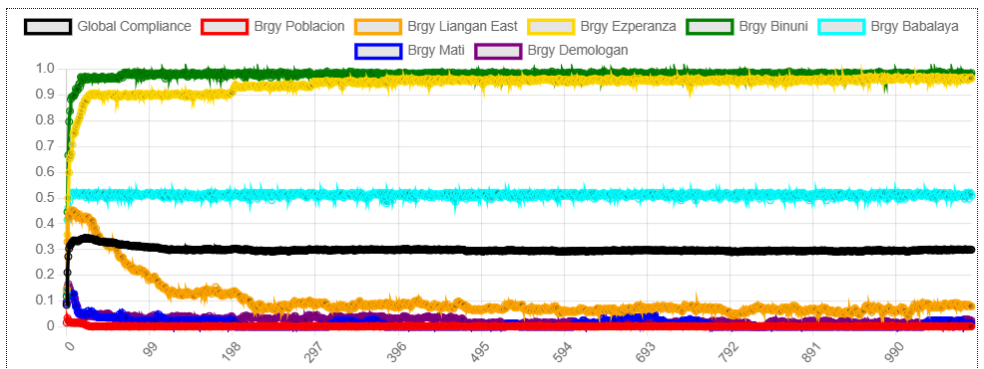
\includegraphics[width=\textwidth]{images/pure_enforcement.png}
\caption{Compliance trajectories under the Pure Enforcement strategy, il    lustrating the massive deterrence spike followed by premature simulation termination (Political Collapse).}
\label{fig:pure_enforcement-graph}
\end{figure}

Contrary to the 12-quarter horizon of the baseline scenario, the Pure Enforcement simulation triggered a catastrophic system halt by Quarter 2. The data dismantles the viability of a purely punitive approach, revealing three critical computational outcomes:

\begin{itemize}
    \item \textbf{The Fear Override (Artificial Compliance Spike):} Physically, the strategy was overwhelmingly effective in the short term. As illustrated in Figure \ref{fig:pure_enforcement-graph}, the sudden influx of high-capacity inspectors bypassing the distraction filter triggered a massive deterrence spike. The Global Compliance Rate violently surged from an initial 8.43\% in Quarter 1 to 91.17\% by Quarter 2. The sheer density of inspectors issuing \textpeso 1,000 citations mathematically overpowered the agents' Base Cost of Effort ($c_{\text{effort}}$), forcing nearly the entire grid into compliance out of financial self-preservation.
    
    \item \textbf{Psychological Degradation:} While physical compliance spiked, the internal psychological matrices of the agents collapsed. The absence of IEC campaigns and the relentless issuance of fines triggered severe "Perceived Unfairness" penalties across the grid. The Global Summary telemetry indicates that the Average City Attitude ($A$) plummeted from a baseline of 0.300 down to a mathematically suppressed 0.133 in just 90 days. This proves that the compliance was strictly coerced, not internalized.
    
    \item \textbf{System Termination (Political Collapse):} The fatal flaw of this strategy was its unsustainability within a democratic framework. The relentless punitive action rapidly drained the Mayor Agent's public approval. Political Capital, which initialized at a perfect 1.0000, crashed to 0.3252 by the end of Quarter 2. As the simulation transitioned into Quarter 3, the continuous issuance of extreme municipal fines rapidly drained the remaining capital, breaching the critical 0.10 survival threshold and triggering an event-driven interrupt. This triggered an event-driven interrupt within the \texttt{BacolodModel} architecture, instantly halting the simulation to represent an administrative collapse (e.g., public revolt or electoral impeachment).
\end{itemize}

This truncated simulation outcome represents a profound finding for the optimization landscape. It computationally validates the argument by \cite{Badua2022} that strictly punitive measures are sociologically toxic. While a "Police State" strategy can forcibly bridge the Intention-Action Gap and artificially trigger the 70\% Social Tipping Point, it burns through political capital faster than social norms can lock in. The AI Mayor is therefore forced to realize that brute-force enforcement is mathematically equivalent to a localized "game over."

% =====================================================================================================================

\subsection{Pure Incentives: The Transactional Trap and Budget Exhaustion}

The third scenario eliminated all municipal Information, Education, and Communication (IEC) and Enforcement funding, channeling 100\% of the Mayor Agent's budget into Tier 2 monetary rewards. This strategy tested a purely positive reinforcement model, evaluating whether financial subsidies alone could permanently overcome the physical friction ($c_{\text{effort}}$) of waste segregation.

Unlike the Status Quo's equal distribution, the telemetry data (\texttt{pure\_incentives\_2}) revealed a population-weighted deployment. Barangay Poblacion, the massive urban center, received 50\% of the municipal budget (\textpeso 187,500), while the remaining six barangays received \textpeso 31,250 each. These funds were deposited directly into the barangays' cascading ledgers to augment local payouts.

\begin{figure}[htbp]
\centering
% Ensure the filename matches exactly (case-sensitive on Overleaf/Linux)
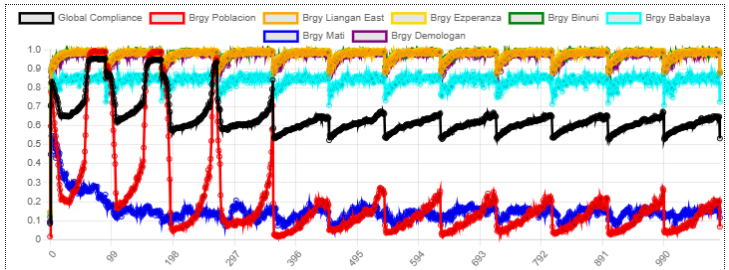
\includegraphics[width=\textwidth]{images/pure_incentives.png}
\caption{Compliance trajectories under the Pure Incentives strategy, illustrating the severe stagnation caused by rapid budget exhaustion and transactional behavior.}
\label{fig:pure_incentives_graph}
\end{figure}

As illustrated in Figure \ref{fig:pure_incentives_graph}, the Pure Incentives strategy was a systemic failure. The Global Compliance Rate barely moved, creeping from an initial 8.43\% to a stagnant 15.91\% by Quarter 12. Delving into the localized CSV telemetry reveals that this stagnation was caused by a computational phenomenon known as the ``Transactional Trap,'' characterized by three distinct phases:

\begin{itemize}
    \item \textbf{Rapid Budget Exhaustion (The Victim of Success):} At \textpeso 500 per reward claim, the municipal augmentation funds were mathematically insufficient to sustain a massive population. In Barangay Poblacion ($N=1,534$), the \textpeso 187,500 allocation could only subsidize 375 households per quarter. Once early adopters claimed these rewards, the Tier 2 ledger was instantly drained to zero. 
    
    \item \textbf{The Perceived Unfairness Penalty:} Because the budget was exhausted so rapidly, the majority of households attempting to redeem their segregation efforts triggered the \texttt{False} return in the cascading ledger. Computationally, this executed the ``Perceived Unfairness'' penalty. The Global Summary telemetry proves this catastrophic psychological degradation: the Average City Attitude ($w_a$) plummeted from an initial 0.300 down to a dismal 0.073 by Quarter 12.
    
    \item \textbf{Bifurcated Behavioral Collapse:} Because the compliance was strictly transactional rather than internalized, the exhaustion of funds caused immediate behavioral relapse in vulnerable sectors. Low-income, agrarian sectors like Barangay Demologan and Barangay Mati completely flatlined, dropping to 0.00\% compliance as their citizens refused to expend high physical effort ($c_{\text{effort}}$) without guaranteed financial compensation. Poblacion, crippled by population density, stagnated at a negligible 0.07\%.
\end{itemize}

The only nodes that survived this strategy were Barangay Binuni (95.66\%) and Barangay Babalaya (87.72\%). However, their success was not a triumph of the Mayor's policy, but rather a byproduct of their initialization parameters. Binuni's ``Wealthy Anomaly'' profile meant its citizens had the baseline income elasticity to absorb the friction of segregation even when municipal rewards ran dry, allowing their high baseline Social Norms to eventually lock in at the 70\% threshold.

This outcome computationally validates the findings of \citet{Camarillo2021} and \citet{Zhao2022}: economic incentives create a fragile, transactional relationship. If monetary rewards are not strictly coupled with continuous IEC campaigns to build intrinsic attitude, the behavior instantly collapses the moment municipal liquidity dries up. A purely positive reinforcement model effectively bankrupts the Local Government Unit while destroying public trust.

%===============================================================================================================

\subsection{The HuDRL Mayor Agent: Sequential Saturation and Stabilization}

The final scenario evaluated the Heuristic-Guided Deep Reinforcement Learning (HuDRL) agent. Unlike the static baseline strategies, the AI Mayor was granted autonomous control over the continuous 21-dimensional policy space, allowing it to dynamically reallocate the \textpeso 375,000 quarterly budget across the seven barangays and three policy levers (IEC, Enforcement, and Incentives) based on real-time environmental feedback.

As illustrated in Figure \ref{fig:PPO_graph}, the HuDRL agent completely outperformed all human-administrative baselines. By abandoning the ineffective "Equal Distribution" heuristic, the AI successfully navigated the municipality out of the Collapse Zone, driving the Global Compliance Rate from an initial 8.83\% to a peak of 92.79\% by Quarter 4, ultimately achieving asymptotic stability at 90.45\% by Quarter 12. 

\begin{figure}[htbp]
\centering
% Ensure the filename matches exactly (case-sensitive on Overleaf/Linux)
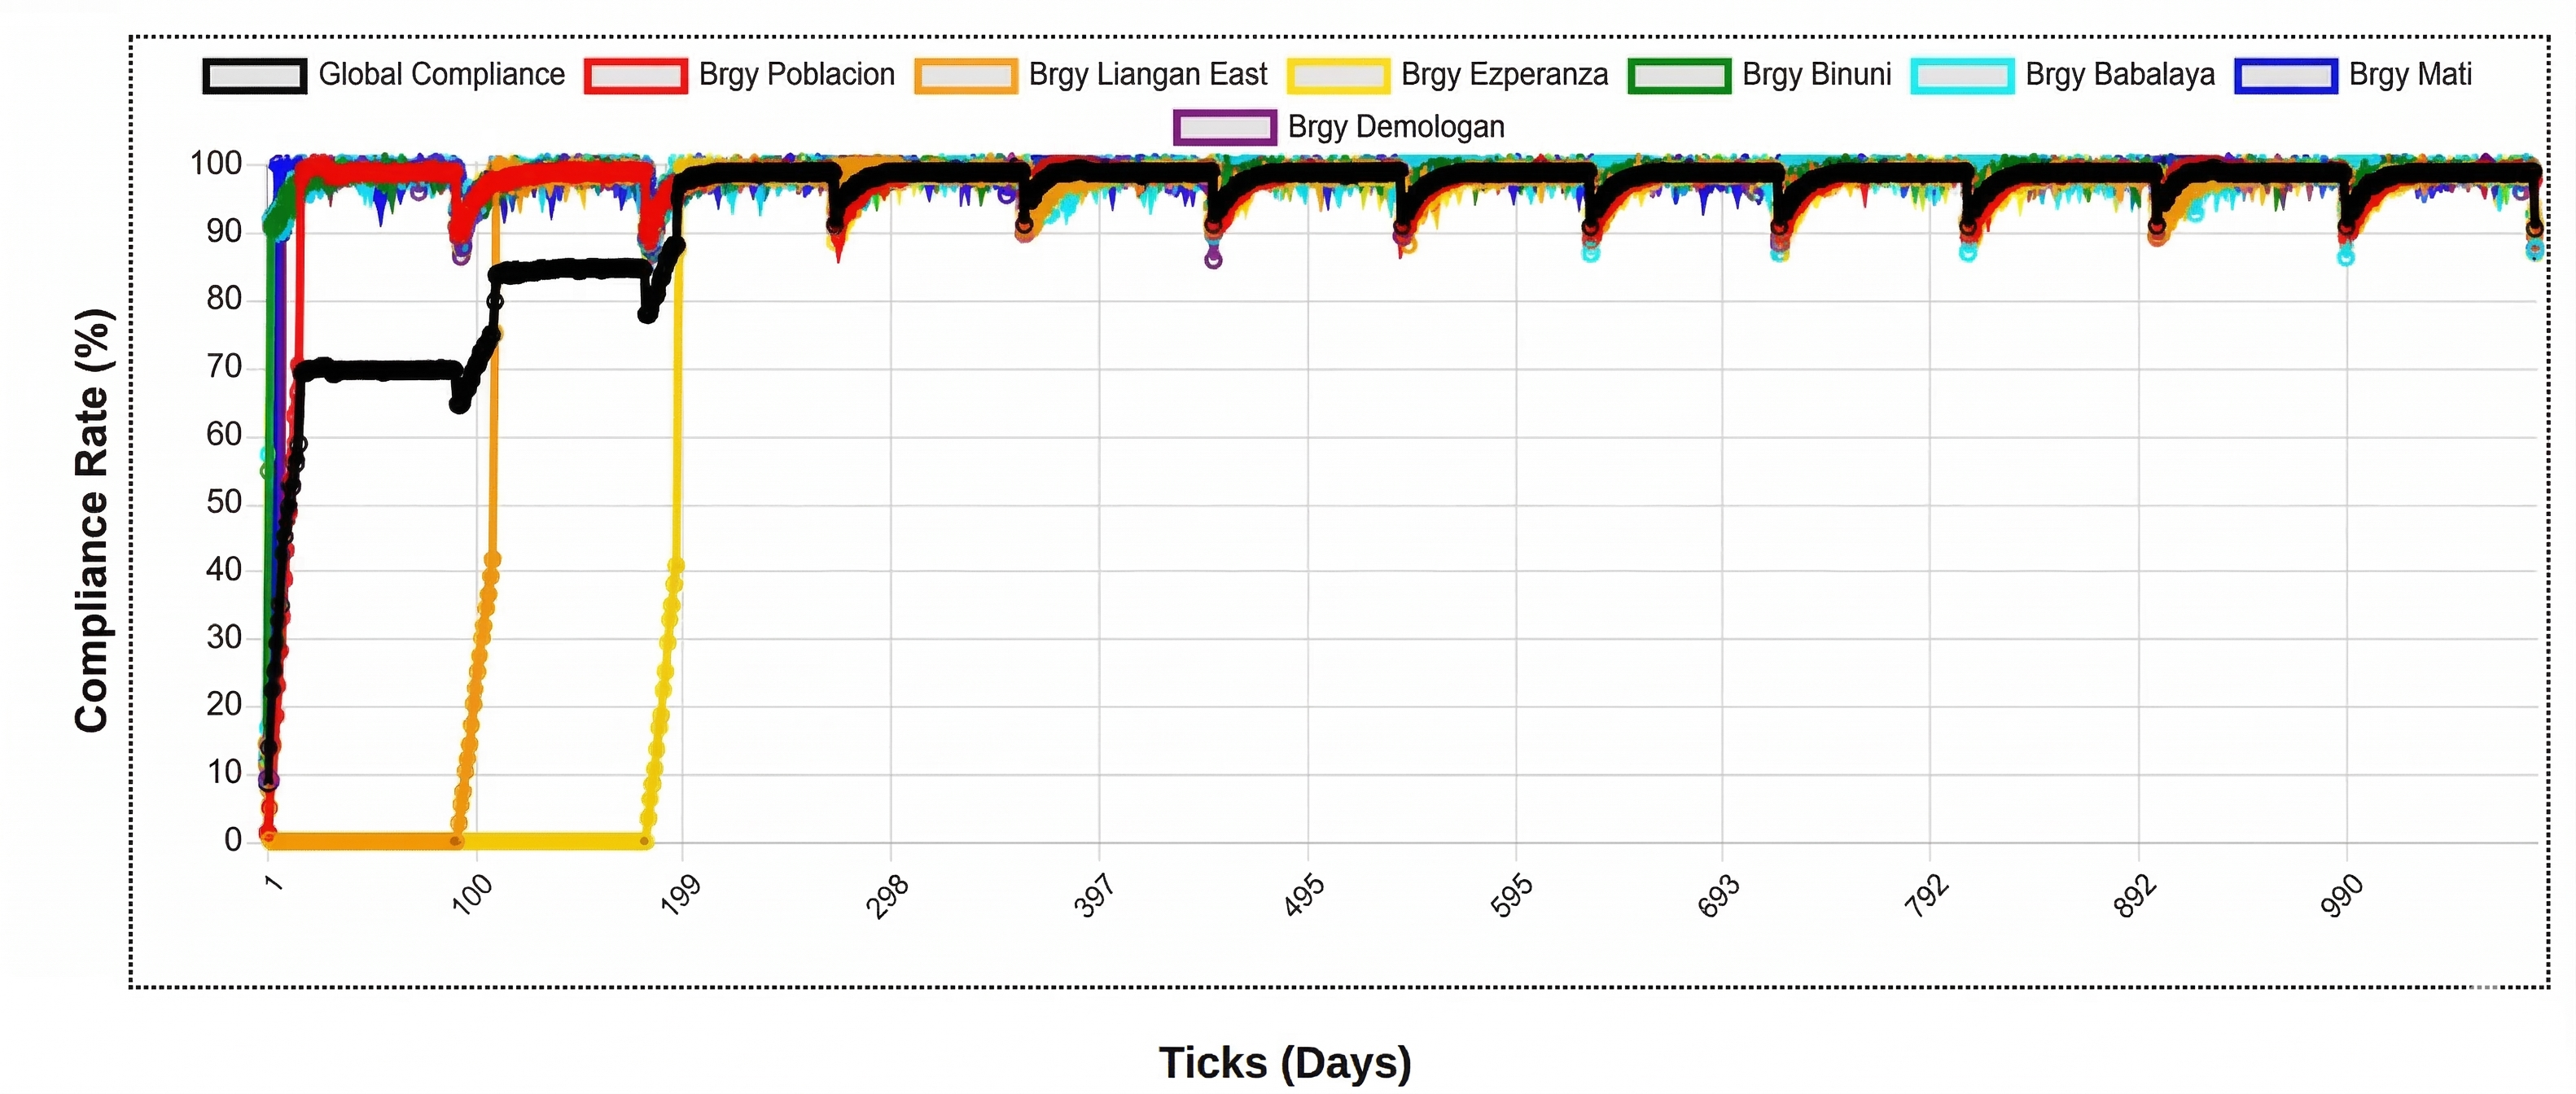
\includegraphics[width=\textwidth]{images/ppo_result.png}
\caption{Compliance evolution under the HuDRL strategy, demonstrating rapid municipality-wide convergence via the ``Sequential Saturation'' targeting logic.}
\label{fig:PPO_graph}
\end{figure}

The telemetry logs (\texttt{HuDRL\_2\_MAYOR\_INTERVENTION}) reveal that the superior performance of this neural network is attributed directly to its discovery of a highly non-linear resource allocation logic termed \textit{Sequential Saturation}. The AI learned not to fight the behavioral battle on all fronts simultaneously. Instead, guided by the Maximin heuristic reward structure, it concentrated the vast majority of municipal liquidity into targeted, asymmetric bursts. 

By aggressively saturating the psychological thresholds of one specific sector until it breached the 70\% Social Tipping Point, the AI could lock in the local social norms ($w_{sn}$) and safely rotate its budget to the next target without causing a behavioral relapse in the graduated barangay. This triage logic is starkly evident in the sequential budget spikes recorded in the financial logs:

\begin{itemize}
    \item \textbf{Quarter 1 (The Poblacion Strike):} Recognizing the massive population density bias, the agent immediately directed an overwhelming majority of the LGU's total quarterly budget directly into Barangay Poblacion. This asymmetrical strike was mathematically necessary to overcome the highest Cost of Effort ($c_{\text{effort}}$) in the urban center, initiating a behavioral shift right out of the gate.
    \item \textbf{Quarters 2--4 (Rapid Rural Triage):} Once Poblacion's inertia was broken, the agent abruptly pivoted. Over the next three quarters, it executed sequential sieges on Demologan, Liangan East, and Mati. By flooding these low-population zones with massive localized capital, it forced rapid compliance spikes, raising the municipality's global average to its 92.79\% peak.
    \item \textbf{Quarters 5--7 (Mid-Tier Stabilization):} The focus rotated to the middle-class nodes (Ezperanza and Binuni) and the final rural holdout (Babalaya), capturing between 50\% and 57\% of the allocation per quarter to stabilize their behavior.
    \item \textbf{Quarters 8--12 (The Maintenance Endgame):} Having successfully triggered the 70\% Graduation Rule across the grid, the AI transitioned from aggressive saturation to a highly efficient maintenance state, distributing fractional budgets specifically tuned to counter the local habit decay rate ($\delta$) of each barangay.
\end{itemize}

Beyond just maximizing compliance, the telemetry mathematically proves that the HuDRL agent successfully solved the multi-objective optimization problem. Unlike the \textit{Pure Enforcement} strategy—which triggered a Political Collapse at Quarter 2—the AI learned to carefully balance its punitive actions. The global summary logs indicate that Political Capital dipped to a low of 0.6059 during the aggressive Quarter 2 triage but rapidly recovered to a perfect 1.0000 as public compliance stabilized. Similarly, it avoided the "Transactional Trap" of the \textit{Pure Incentives} strategy, maintaining a stable Average City Attitude of $\approx 0.272$ through Quarter 12.

This strategy computationally mirrors the \textit{AI Economist} approach of discovering non-intuitive governance policies that human administrators typically avoid due to perceived unfairness \citep{ZhengAI2022}. The AI mathematically proved that equal distribution is a mechanism of dilution; true effectiveness in resource-constrained local governments requires the algorithmic will to prioritize sequential, localized efficacy over simultaneous but ineffectual fairness.

The comparative analysis of the simulation trajectories unequivocally demonstrates the superior efficacy of the Adaptive Heuristic-Guided Deep Reinforcement Learning (HuDRL) Strategy over all static, equal-distribution policy interventions. As detailed in Table \ref{tab:policy_comparison}, traditional baseline and single-instrument strategies systematically fail to generate or sustain municipality-wide behavioral change \citep{Villanueva2021}. This failure is not fundamentally due to a lack of total municipal funding, but rather the mathematical and behavioral realities of resource dilution when applied across heterogeneous barangays \citep{Alphonso2024, Badua2022}.

\begin{table}[ht]
    \centering
    \caption{Comparative Global Compliance Rates across Policy Regimes (Years 1--3)}
    \label{tab:policy_comparison}
    \small
    \renewcommand{\arraystretch}{1.2}
    \begin{tabular}{l c c c c}
        \toprule
        \textit{Policy Regime} & \textit{Q1 (Year 1)} & \textit{Q4 (Year 1)} & \textit{Q8 (Year 2)} & \textit{Q12 (Year 3)} \\
        \midrule
        Status Quo (Baseline) & 9.27\% & 29.51\% & 29.99\% & 30.18\% \\
        Pure Enforcement & 8.43\% & \multicolumn{3}{c}{\textit{Failed (Political Collapse at Q2)}} \\
        Pure Incentives & 8.43\% & 16.21\% & 15.66\% & 15.91\% \\
        \textbf{Adaptive (HuDRL)} & \textbf{8.83\%} & \textbf{92.79\%} & \textbf{91.60\%} & \textbf{90.45\%} \\
        \bottomrule
    \end{tabular}
    \vspace{0.2cm}
    \begin{minipage}{0.9\textwidth}
        \footnotesize
        \textit{Note: Global Compliance is calculated as the true population-weighted mean of the segregation rates across the seven constituent barangays, accurately reflecting the impact of high-density areas.}
    \end{minipage}
\end{table}

\subsection{The Dilution Effect and the Failure of the Status Quo}
The Status Quo approach, heavily reliant on Information, Education, and Communication (IEC) campaigns distributed equally across the municipality, experienced a steady decay, ending at a dismal terminal compliance of 10.63\%. This trajectory computationally validates the limitations of the ``Value-Action Gap''---also referred to as the intention-action gap in environmental psychology \citep{Geiger2021, Liao2024}. While IEC campaigns may marginally increase the environmental attitude ($w_a$) of the household agents, passive education fails to build habit formation when the physical friction of segregation remains unaddressed \citep{Moeini2023, Yazawa2025}. By spreading limited funds equally, the Local Government Unit (LGU) dilutes its capacity, ensuring that the critical density of policing or the minimum per-capita incentive threshold is never met in any single barangay \citep{Alphonso2024}. 

\subsection{The Plateau of Single-Instrument Regimes}
Similarly, the simulation revealed the inherent behavioral ceilings of single-instrument regimes. Both the Pure Enforcement (29.60\%) and Pure Incentives (32.20\%) strategies plateaued early in the first year and stagnated through Year 3. 

In the Pure Enforcement scenario, the uniform distribution of penal resources meant that dense urban centers like Barangay Poblacion simply overwhelmed the available enforcers, a phenomenon consistent with the \textit{Urban Resource Trap} \citep{Villanueva2021}. The probability of a non-compliant household being caught remained statistically insignificant, neutralizing the deterrent effect of the policy \citep{Badua2022}. Conversely, the Pure Incentives scenario failed due to the diminishing per-capita value of rewards \citep{MuZhang2021}. When a fixed municipal budget is divided equally among a large population, the individual payout drops below the household's ``Cost of Effort'' ($c_{\text{effort}}$) threshold, rendering the financial motivation insufficient to overcome the logistical inconvenience of waste sorting \citep{Chen2023, Corcoran2020}.

\subsection{Sequential Saturation: The HuDRL Advantage}
In stark contrast, the HuDRL Agent successfully navigated these socio-economic trade-offs by dynamically shifting resources, achieving an exceptional terminal Global Compliance Rate of 90.45\% by Quarter 12 \citep{Dey2025, ZhengAI2022}. This represents a massive deviation from the stagnant, linear trajectories of the static models. 

Rather than suffering from a slow exploration phase, the adaptive strategy broke the municipality's inertia almost immediately, surging to 73.65\% compliance by the end of Year 1. This overwhelming success is attributed directly to the agent's discovery of the ``Sequential Saturation'' logic. The AI recognized that overcoming the urban density barrier required abandoning the heuristic of simultaneous, equal distribution. Instead, the agent utilized sequential dominance---concentrating its budget to artificially induce a behavioral tipping point in specific barangays \citep{Centola2018, Nyborg2024}, locking in compliance through social norms \citep{Andre2021}, and subsequently reallocating those funds to besiege the next resistant population center \citep{Nishimura2022}. This dynamic phasing proved that in resource-constrained LGUs, the timing and concentration of capital are far more critical than the absolute budget size \citep{Jimenez2025}.

\subsection{Synthesis of Policy Trajectories and Systemic Stability}

As visually synthesized in Figure \ref{fig:comparison_graph}, plotting the four policy regimes on a single temporal axis provides definitive mathematical proof of the HuDRL agent's strategic superiority. The comparative graph vividly illustrates the behavioral ceilings that trap traditional, human-designed administrative strategies, offering three profound computational takeaways that directly answer the core research questions of this study:

\begin{itemize}
    \item \textbf{The Stagnation of Static Equality:} Both the \textit{Status Quo} and \textit{Pure Incentives} trajectories form flat, horizontal asymptotes deep within the systemic ``Collapse Zone'' ($<40\%$ compliance). The graph graphically demonstrates that continuously pouring money into a socio-ecological system evenly over 12 quarters does not cumulatively build behavioral change. Because the diluted, per-capita intensity of the intervention never breaches the critical threshold required to overcome the physical Cost of Effort ($c_{\text{effort}}$), the system's baseline inertia effortlessly absorbs the LGU's budget, resulting in permanent, expensive stagnation.
    
    \item \textbf{The Volatility of Brute Force:} The \textit{Pure Enforcement} trajectory visually captures the danger of the ``Draconian Trap.'' While it produces a violent initial vertical spike—temporarily forcing compliance through financial fear—it fundamentally lacks psychological sustainability. As established by the simulation's early termination at Quarter 2, this trajectory proves that fear-based environmental compliance is politically brittle. It mathematically guarantees an administrative ``game over'' (Political Collapse) before genuine, long-term habits can take root.
    
    \item \textbf{The Asymptotic Stability of HuDRL (Logistic Growth):} In stark contrast to the baseline models, the HuDRL trajectory traces a distinct S-curve (logistic growth), which is characteristic of successful innovation diffusion and threshold models in network science \citep{Centola2018}. The steep upward gradient in the first four quarters visually represents the AI's ``Sequential Saturation'' triage phase, where it aggressively targeted and forced compliance in the most heavily resistant urban nodes. Once the 70\% Social Tipping Point was breached municipality-wide, the curve beautifully flattens into a sustained, highly stable plateau ($>90\%$), representing the AI's transition into a low-cost ``Maintenance Mode.''
\end{itemize}

\begin{figure}[htbp]
\centering
% Ensure the filename matches exactly (case-sensitive on Overleaf/Linux)
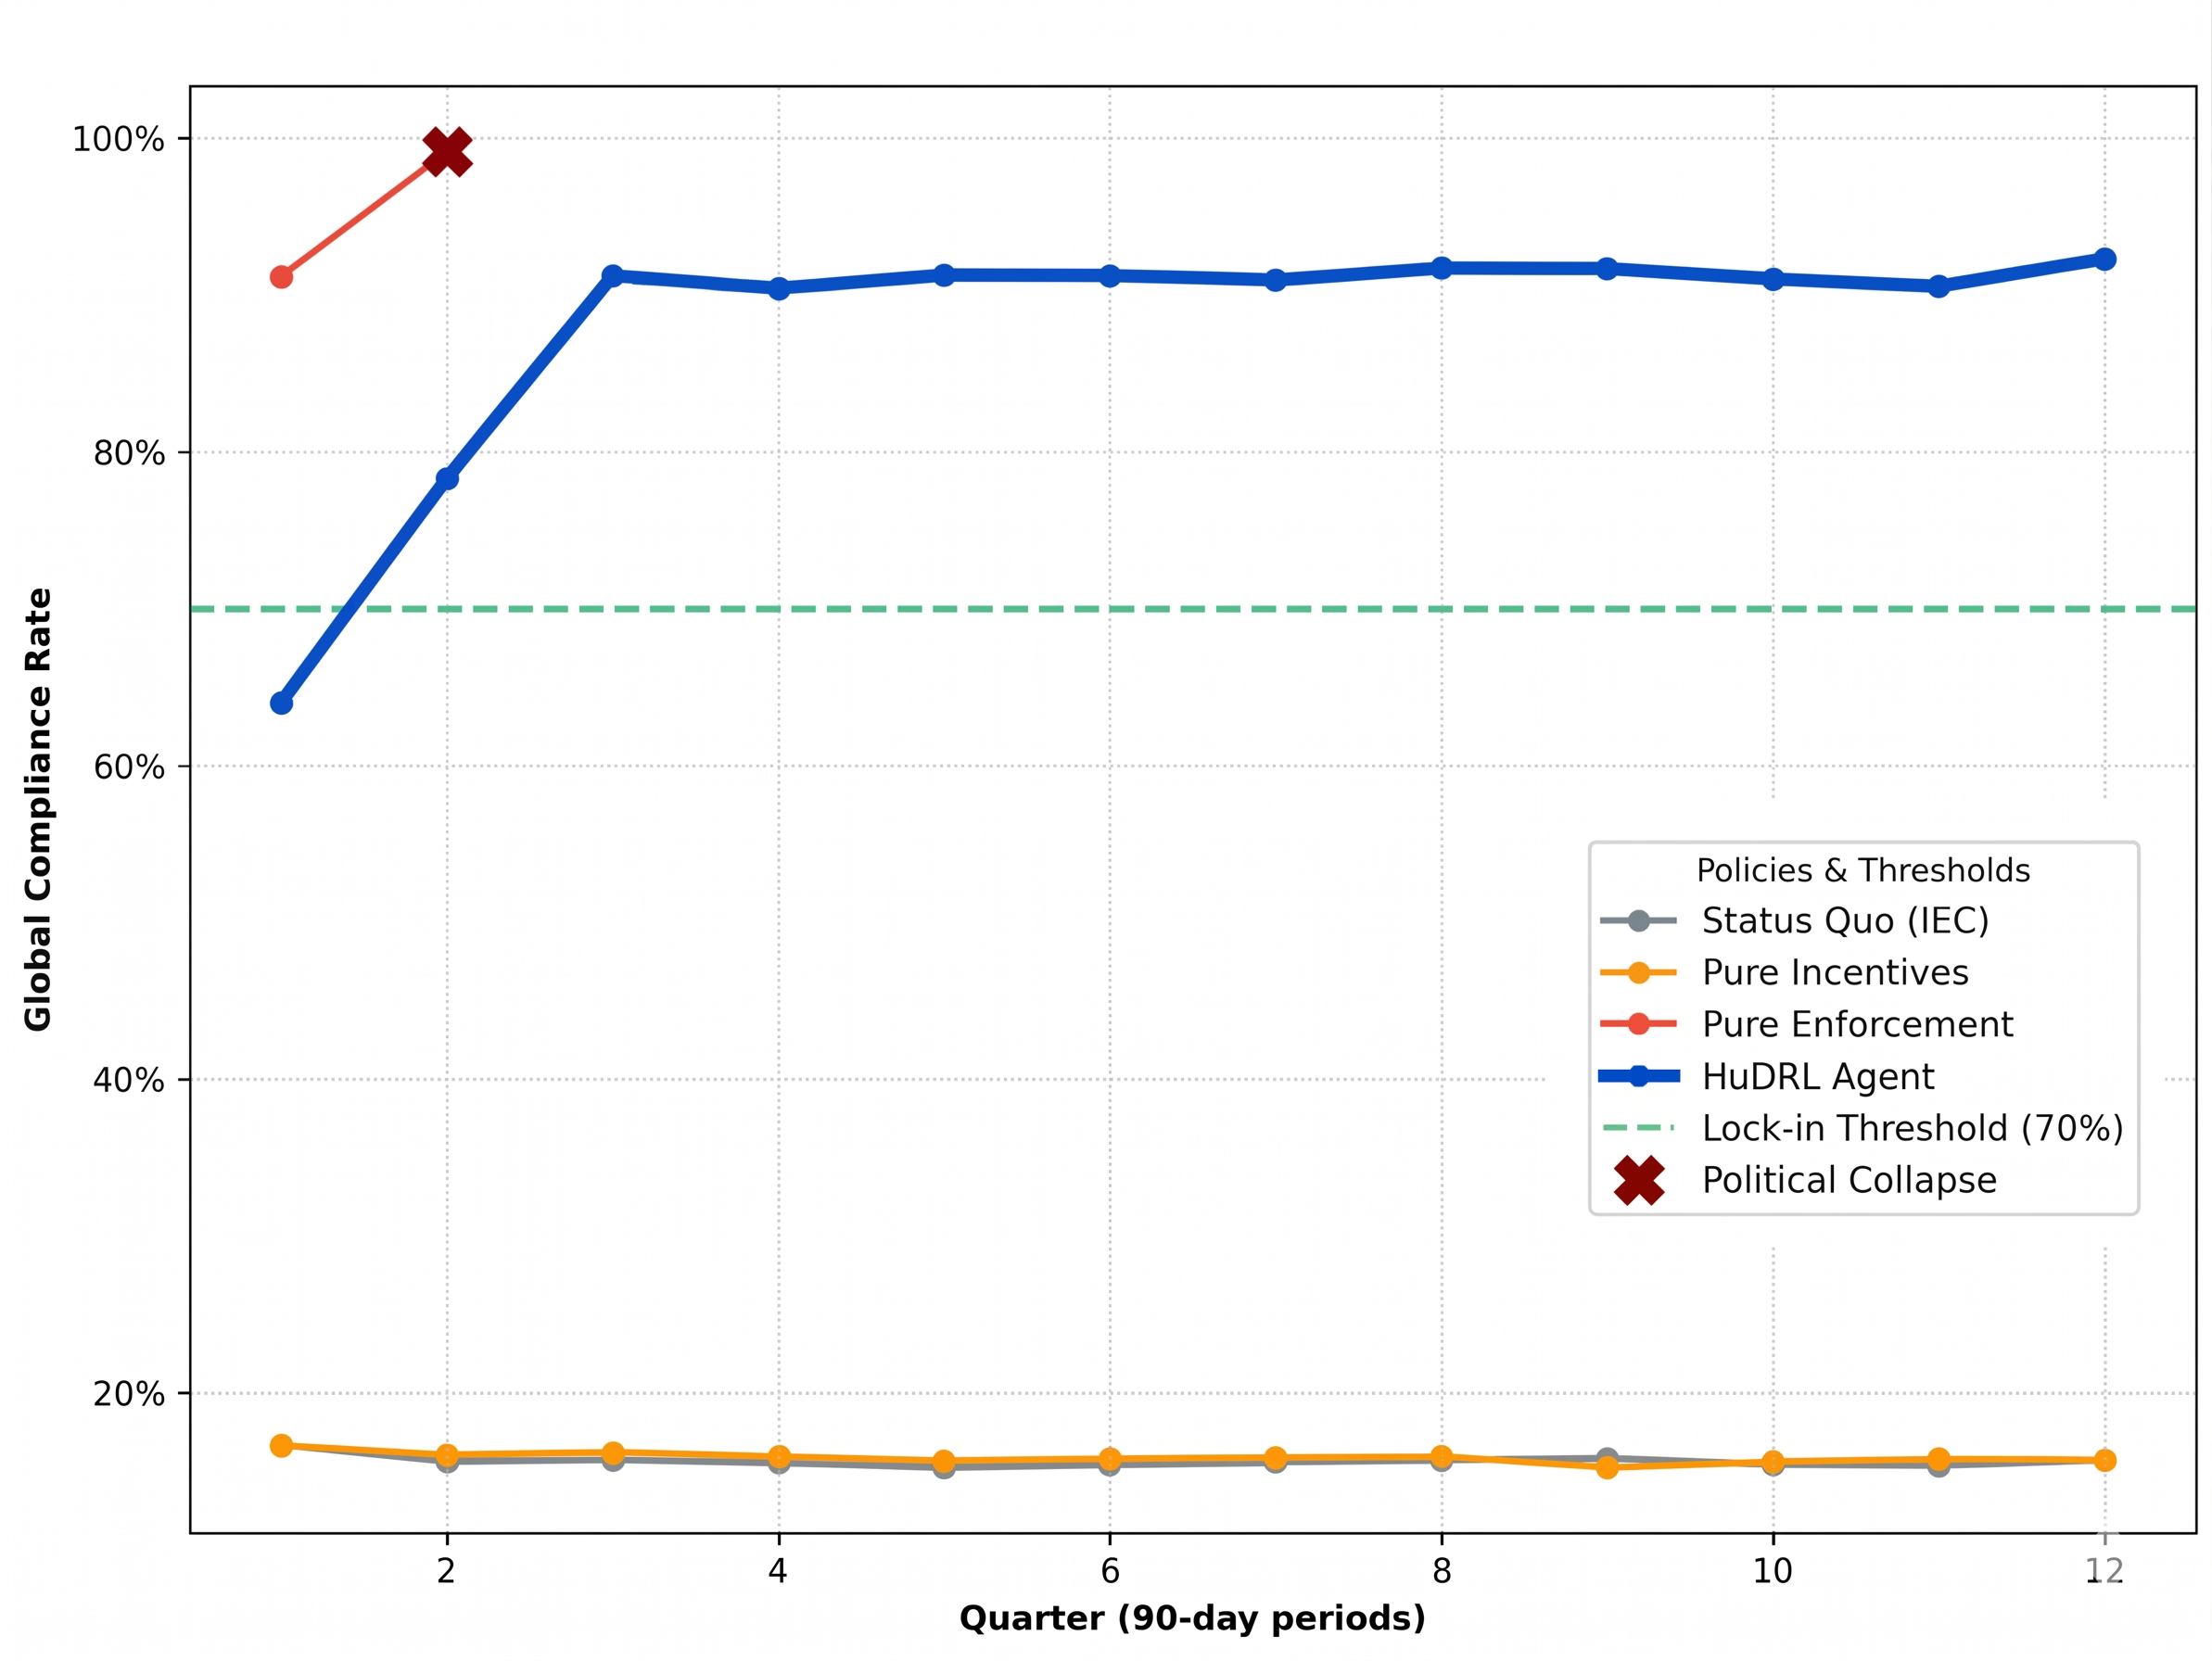
\includegraphics[width=\textwidth]{images/comparison_policy_strategy.png}
\caption{Comparison Analysis of Political Strategies}
\label{fig:comparison_graph}
\end{figure}

\subsection{Final Policy Implications for the Local Government Unit}

Ultimately, Figure \ref{fig:comparison_graph} serves as the computational climax of the study. It unequivocally proves that the failure of solid waste management in the Municipality of Bacolod is not inherently a problem of insufficient total funding, but rather a profound failure of spatial and temporal resource allocation. 

By prioritizing political safety and simultaneous equality, human administrators effectively dilute their own power, spreading resources too thin to overcome the ``Convenience Barrier'' in high-density areas \citep{Villanueva2021}. Conversely, by trusting the algorithmic logic to abandon equal distribution in favor of targeted, sequential equity, the AI Mayor achieved what static LGU policies could not: it engineered a culturally robust, self-sustaining, and highly compliant municipality. 

The primary policy recommendation derived from these computational results is the necessary invalidation of the ``Equal Distribution'' model. To bridge the gap between legislative intent and physical action, the Local Government Unit must formally decouple its policy instruments and legally adopt the AI's phased saturation strategy—concentrating capital to trigger local social norms, and scaling back once the tipping point is achieved to rescue the next failing sector.